\documentclass[12pt]{article}

\usepackage{graphicx}
\usepackage[spanish]{babel}
\usepackage[utf8]{inputenx}
\usepackage{anysize} 
\usepackage{amsmath}
\usepackage{listings}
\marginsize{2cm}{2cm}{1cm}{2cm} %izq der arriba abajo
\usepackage{hyperref}
\usepackage{wrapfig} % paquete gráfico

\hypersetup{
    colorlinks,%
    citecolor=black,%
    filecolor=black,%
    linkcolor=black,%
    urlcolor=black
}

\title{}
\author{Facundo Nahuel Uriel Silva}

\begin{document}

  %Caratula
  \newpage
  \thispagestyle{empty}
  
  \begin{center}
    
\includegraphics[width=250px]{../../logo_fiuba_alta.jpg} 

  \vspace{100px}

  \huge{Trabajo Profesional de Ingeniería Electrónica}
  \vspace{50px}

  \bf{ \huge{Sistema de control para proceso de sinterizado de nano estructuras \\} }
  \vspace{35px}
  \Large{\textit{ANTEPROYECTO}}

  \vspace{70px}

  \end{center}
  
  \begin{bf}
    \begin{Large}
      \begin{tabbing}
	\= ----- \= ----- \= --------------------- \= \kill
	\> Integrantes:\\
	\\
	  \>\> Estanislao López Morgan \\
	  \>\>\>  Padrón:	\> 84546 \\
	  \>\>\>  Mail:	\>\url{estanux@gmail.com} \\
	\\
	  \>\> Facundo Nahuel Uriel Silva\\
	  \>\>\>  Padrón:	\> 86881 \\
	  \>\>\>  Mail:	\> \url{fanaur@gmail.com}\\
      \end{tabbing}
    \end{Large}
  \end{bf}
    
  %Indice de contenidos
  %\newpage
  
  
  \thispagestyle{empty} \tableofcontents \thispagestyle{empty} %así se hace el número de página

  %Comienzo
  \newpage
  \setcounter{page}{1}

%--------------------------------------------------------------------------------------------------------------------  
%--------------------------------------------------------------------------------------------------------------------

  \section{Introducción}  
%.....Para que la figura salga al lado del texto........

\begin{wrapfigure}{r}{0.5\textwidth}
  \begin{center}
   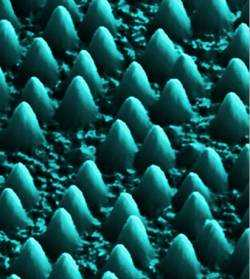
\includegraphics[width=0.45\textwidth]{../../Diagramas/nanotecnologia02.jpg}
    
  \end{center}
  \caption{Nanoestructura}
\end{wrapfigure}

Los materiales nanocompuestos formados en su totalidad por particulas cerámicas y metálicas en el rango de los centenares
  y decenas de nanómetros, son una clase de materiales que presentan propiedades físicas muy distíntas a las de esos mismos
 con tamaños de cristal micrométricos (materiales convencionales). Tales propiedades, al ampliar su rango de funcionalidad
 resultan muy interesantes desde el punto de vista tecnológico ya que permiten combinar propiedades excepcionales con funcionalidad
 imprescindibles en aplicaciones específicas, como la transparencia, la biocompatibilidad, la dureza o conductividad eléctrica, entre otras.

 Sin embargo, la aplicacion industrial de los materiales nanocompuestos radica en la capacidad de consolidación de estos materiales
 formando cuerpos densos y compuestos, pero preservando el tamañan nanométrico de sus componentes. Las técnicas de consolidación convencionales
 presentan importantes limitaciones y no son capaces de preservar esta nanoestructura. 
 La solución de estos problemas y el desarrollo de nuevas tecnologías ha posibilitado la producción de materiales nanoestructurales.


%--------------------------------------------------------------------------------------------------------------------  
%--------------------------------------------------------------------------------------------------------------------
 \section{Finalidad del proyecto}  
 En el laboratorio de sólidos amorfos de la facultad de ingeniería de la universidad de Buenos Aires funciona el 
 INTECIN y en el mismo el \href{''http://intecin.fi.uba.ar/grupos.php?grupo=12''}{grupo de materiales nanoestructurales}, este grupo prepara y
 estudia sistemas basados en nanopartículas magnéticas apuntando a las posibles aplicaciones tecnológicas
 en sensores, remediación ambiental y aplicaciones clínicas. Sus integrantes tienen experiencia en caracterización estructural por difracción, dispersión y absorción
 de rayos X, espectroscopia Mössbauer, propiedades magnéticas y de magnetotransporte y microscopía electrónica.\newline
  
  Para lograr esto se realiza el sintetizado de nano estructuras, obteniendo una cinta metálica con una estructura amorfa (sin estructura cristalina)
  similar a un vidrio. Mediante un proceso de pulverizado de esta cinta se obtiene un polvo cuyas partículas poseen una estructura nanométrica.
  Para poder obtener una estructura sólida a partir del polvo se utiliza el proceso de sinterizado. Este proceso
  logra unificar las particulas del polvo en una sola estructura sólida. Para este fin se necesita que una intensidad de corriente
  elevada, en el orden de los KA, atraviese la muestra de polvo nonometrico. Esta corriente puede ser provista por un banco de 
  capacitores (proceso rápido) o una fuente de RF (proceso lento).\newline

  La finalidad de nuestro proyecto es desarrollar una automatización y relevamiento del proceso de sinterizado a partir de la 
  descarga de un banco de capacitores, realizar recopilación de datos del proceso con la posibilidad de variar alguna variables
  involucradas en el sitenrizado para evaluar el desempeño del mismo y sus resultados.
 
%--------------------------------------------------------------------------------------------------------------------  
%--------------------------------------------------------------------------------------------------------------------

  \section{Planteamiento del problema a resolver}  

  Para el estudio y desarrollo de cualquier tecnología es indispensable la experimentación, ya que es el medio atraves del cual
  se puede comprender y validar los desarrollos teóricos del proceso estudiado. La flexibilidad a la hora de la experimentación
  es factor deseado, entendiendo por flexibilidad la posibilidad de poder modificar parámetros del experimento de forma rapida y
  sencilla, ya que facilita y ahora tiempos a la hora del desarrollo del conocimiento. La fácil obtención y disponibilidad de 
  los resultados de la experimentación es otro deseado en la experimentación. \newline

  Para poder estudiar y obtener materiales nanometricos atraves del proceso de sinterizado es necesario contar con un plataforma 
  que controle y monitoree el proceso de sinterizado de forma flexible y parametrica. La plataforma le debe brindar al investigador
  la posibilidad de modificar las variables del proceso y obtener los resultados de la experimentacion.
  El proceso de sinterizado requiere la manipulación de una potencia electrica conciderable, es por ello que la plataforma debe	
  brindar un manejo seguro de esta potencia , contando con todas medidas de seguridad requeridas para asegurar una segura operación.

%--------------------------------------------------------------------------------------------------------------------  
%--------------------------------------------------------------------------------------------------------------------

  \section{Análisis de mercado}  

  Los nanomateriales poseen una gran potencialidad a nivel tecnológico, ya que posibilitan la optimización y mejora de actuales
  de materiales actuales.
  Particularmente utilizando el proceso de sinterizado de materiales magneticos se obtiene materiales
  con caracteristicas magneticas conciderablemente mejores que los materiales actualmente usados en la industria.
  Los materiales magneticos son de vital importancia el campo de la generación de energia electrica, almacenamiento electronico de datos, 
  desarrollo de sensores electrónico, etc.
  \newline

    \newpage
%--------------------------------------------------------------------------------------------------------------------
%--------------------------------------------------------------------------------------------------------------------

\section{Análisis de la competencia}  

\vspace{15px}
%\begin{center}
 
\includegraphics[width=200px]{../../Diagramas/logo(1).jpg}
 % logo(1).jpg: 365x63 pixel, 72dpi, 12.88x2.22 cm, bb=0 0 365 63
%\end{center}
\vspace{25px}

\begin{wrapfigure}{r}{0.55\textwidth}
  \vspace{-20px}  
  \begin{center}
    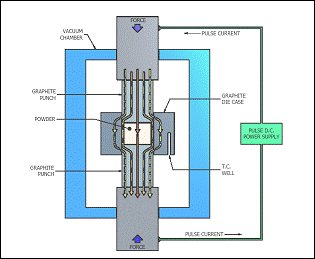
\includegraphics[width=0.4\textwidth]{../../Diagramas/image004.jpg}
  \end{center}
  \caption{SPS}
  \vspace{-20px}
\end{wrapfigure}

En el mercado encontramos soluciones de gran emplazamiento y envergadura, como lo son los propuestos por \href{''http://thermaltechnology.com/index.php?option=com_content&view=article&id=84''}{Thermal Technology LLC}
 basado en la tecnología de Spark Plasma Sintering (SPS) un revolucionario en polvo de alta velocidad de proceso de consolidación.
 SPS utiliza alto pulsos de alta corriente continua para activar la consolidación y la reacción de sinterización de los
 materiales. Un sistesma de SPS trabaja con materiales conductores, no conductores y compuesto a cualquier nivel de densidad.
 La ventaja de SPS es ahorro de tiempo y energía y la capacidad de retener nanoestructuras.
 

%--------------------------------------------------------------------------------------------------------------------  
%--------------------------------------------------------------------------------------------------------------------

  \section{Planes de crecimiento}  
El proyecto en un principio propone realizar la automatización del proceso de sinterizado estableciendo las normas de seguidad
que corresponden. En un segundo paso, realizar las medeciones sobre las mágnitudes involucradas en el proceso. Tensión, corriente
tiempo de descarga, etc, y su posterior almacenamiento. Finalmente todo lo anterior se lo integraría de forma que pueda sincronizar
contra un servidor en red.

%--------------------------------------------------------------------------------------------------------------------  
%--------------------------------------------------------------------------------------------------------------------

  \section{Objetivos de costo}  
El objetivo propuesto trata de desarrollar instrumental de bajo o mediano costo en comparación a las opciones propuestas por
la competencia. Desde ese punto de vista, el proceso de sinterizado a través de descarga de los capacitores propuesto es mas 
eficiente

%--------------------------------------------------------------------------------------------------------------------  
%--------------------------------------------------------------------------------------------------------------------

  %\section{Factores de desempeño}  

%--------------------------------------------------------------------------------------------------------------------

\end{document}
